\documentclass[a4paper,12pt]{article}


\usepackage{graphicx}
\usepackage{tikz}
\usetikzlibrary{positioning, arrows.meta}
\usepackage{amsmath}   
\usepackage{caption}       
\usepackage{xepersian}
\usepackage{setspace}
\usepackage{perpage}
\MakePerPage{footnote}
\usepackage{multirow}



\renewcommand{\contentsname}{فهرست مطالب\\}
\numberwithin{figure}{subsection}
\settextfont[Extension=.ttf]{IRNazanin}

\begin{document}

\begin{titlepage}

    \centering
   \vspace*{-3cm}
    
    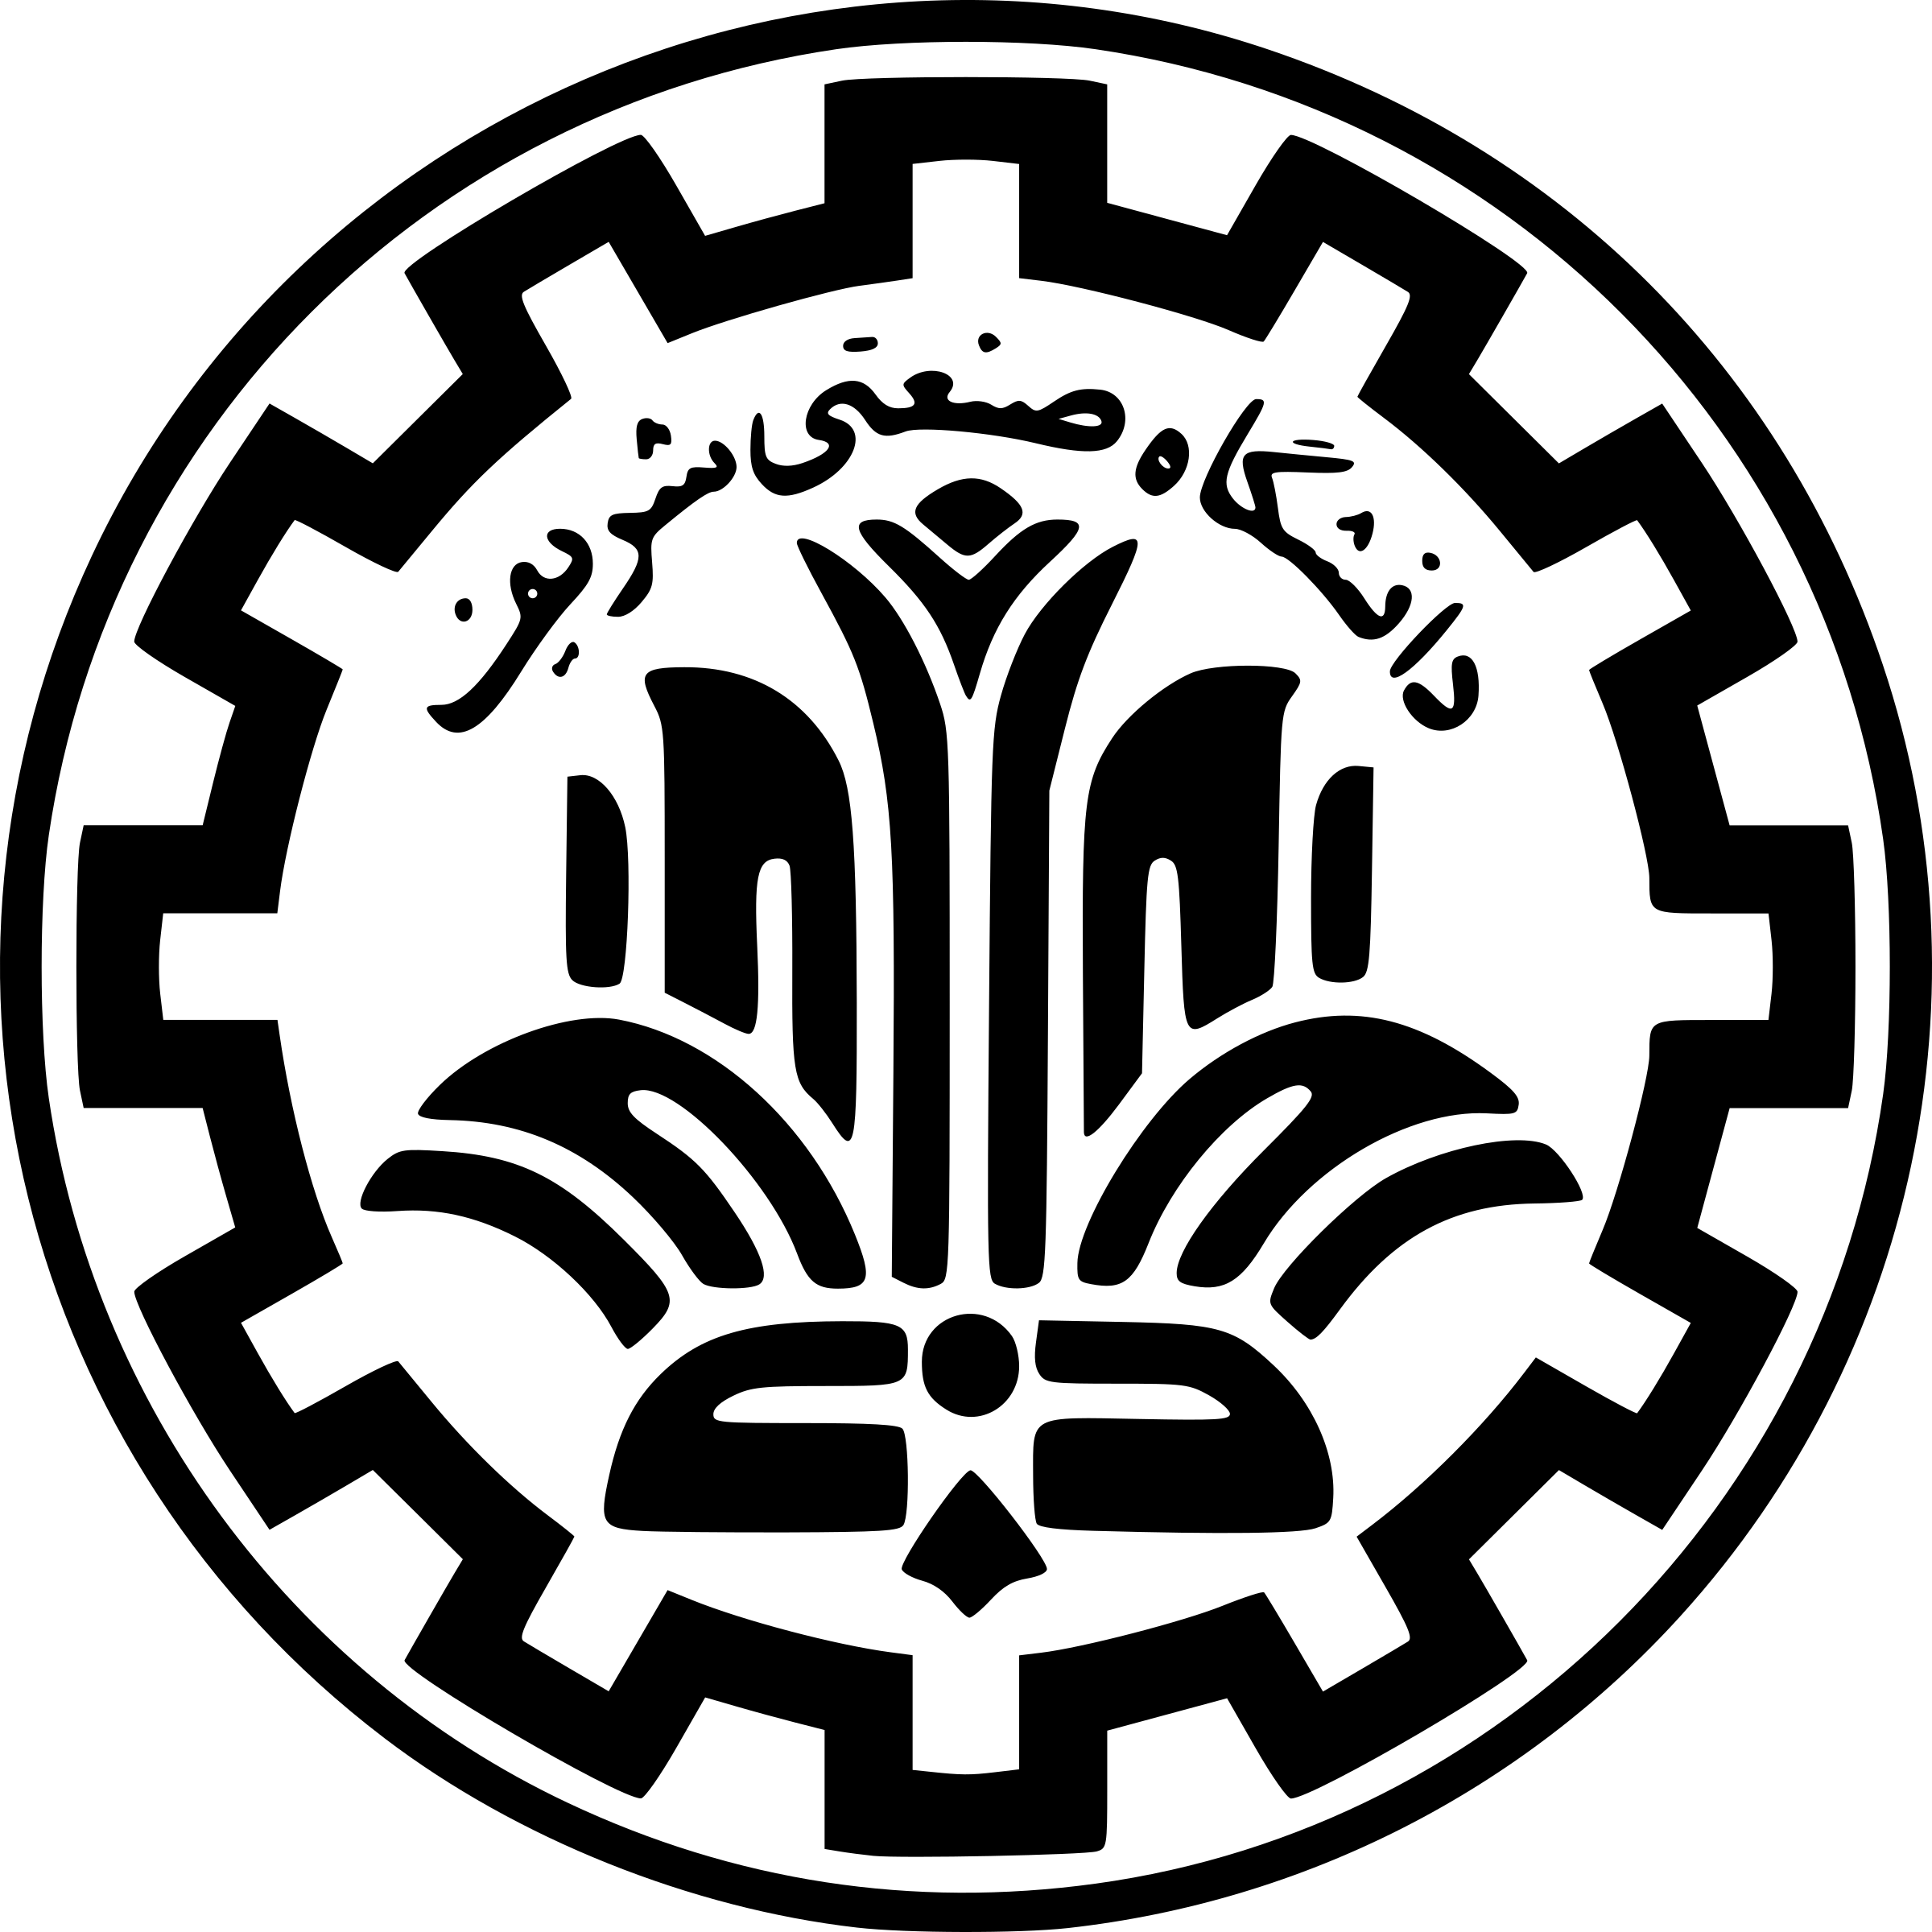
\includegraphics[width=4cm]{images/logo.png} 
    \\[1cm] 
    
    
    {\Large \textbf{گزارش آزمایش}}\\[0.3cm]
    {\Large آزمایشگاه مدار منطقی}\\[1.5cm]
    
    {\LARGE \textbf{آزمایش چهارم}}\\[0.5cm]
    {\huge \textbf{مدار کنترل‌کننده}}\\[2.5cm]
    
    
    \begin{table}[h]
        \centering
        \large
        

        اعضای گروه:\\
        \vspace{0.5cm}
        \renewcommand{\arraystretch}{1.5} 
        \begin{tabular}{|c|c|}
            \hline
            \textbf{نام و نام خانوادگی} & \textbf{شماره دانشجویی} \\
            \hline
           روناک ابوطالبی & 404105394 \\
            \hline
            حسین مرادی & 404106366 \\
            \hline
        \end{tabular}
    \end{table}
    
    \vspace{2.5cm}
    
    {\large \textbf{تاریخ تحویل: 1405/06/04}}\\[1cm]
    
    {\large \textbf{تابستان 1405}}\\[1cm]
    
    \vfill
    
\end{titlepage}

\newpage
\begin{spacing}{1.5} 
    \tableofcontents 
\end{spacing}

\newpage

\section{مقدمه و تعریف مسئله}
\leavevmode\par
\vspace{0.3cm}

\begin{spacing}{1.3}
هدف از این آزمایش ساخت دو مدار کنترل‌کننده ساده با کمک \lr{ASM Chart} و پیاده‌سازی آنها به کمک نرم‌افزار \lr{Proteus} است. مدارهای کنترل‌کننده نقش هسته مرکزی را در سیستم‌های دیجیتال ایفا می‌کنند و وظیفه آن‌ها تولید سیگنال‌های کنترلی مناسب بر اساس ورودی‌ها و وضعیت فعلی سیستم است.

در این گزارش کار، برخلاف روال معمول که تنها یکی از پروژه‌ها انتخاب می‌شود، طراحی و شبیه‌سازی هر دو مدار کنترلی زیر به طور کامل و جامع انجام پذیرفته است:

\begin{itemize}
    \item \textbf{تایمر یک ماشین لباس‌شویی:} در این بخش، یک مدار کنترل‌کننده برای یک ماشین لباس‌شویی با دو برنامه شست‌وشو با آب گرم و سرد طراحی شده است. این سیستم با دریافت سیگنال‌های ورودی مانند وضعیت شیر آب (\lr{Valve})، بسته بودن در (\lr{Door})، کلید شروع (\lr{Start}) و نوع برنامه (\lr{Function})، خروجی‌ها و عملیات مختلفی نظیر آب‌گیری (\lr{Fill})، گرم کردن (\lr{Heat})، شست‌وشو (\lr{Wash})، تخلیه (\lr{Drain}) و خشک کردن (\lr{Dry}) را طی زمان‌بندی‌های مشخص مدیریت می‌کند.
    
    \item \textbf{تلفن راه‌دور:} پروژه دوم به طراحی مدار کنترل‌کننده یک تلفن عمومی اختصاص دارد که با دریافت سکه‌های ده ریالی کار می‌کند و تعداد سکه‌های موجود را بر روی دو عدد نمایشگر ۷ قطعه‌ای نشان می‌دهد. کنترل‌کننده وظیفه دارد پس از انداختن حداقل یک سکه و فشردن کلید شروع (\lr{Start})، تماس را برقرار کرده (\lr{Call}) و با گذشت زمان بر اساس پالس ساعت، موجودی را کسر کند. همچنین در صورت به صفر رسیدن موجودی، سیستم هشدار (\lr{Alarm}) را روشن کرده و در صورت عدم افزایش سکه در زمان مشخص، تماس تلفنی را قطع می‌نماید.
\end{itemize}

در ادامه این گزارش، مراحل طراحی شامل رسم نمودار \lr{ASM}، تعیین وضعیت‌ها، استخراج معادلات و در نهایت پیاده‌سازی و شبیه‌سازی این دو مدار در محیط \lr{Proteus} مورد بررسی قرار خواهد گرفت.
\end{spacing}

\newpage


\section{تایمر ماشین لباسشویی}
\leavevmode\par
\vspace{0.3cm}

\subsection{بررسی و انتخاب روش طراحی}
\leavevmode\par
\vspace{0.2cm}

\begin{spacing}{1.3}

از آنجا که یکی از اهداف این آزمایش آشنایی با \lr{ASM Chart} و طراحی به کمک آن است، ابتدا \lr{ASM Chart} مناسب برای مدار رسم می‌کنیم.

برای طراحی \lr{ASM Chart}، با تعریف حالت‌های مورد نیاز شروع می‌کنیم و با شروع از حالت پایه و در نظر گرفتن انتقالات بین حالات بر اساس مقادیر ورودی مختلف، آن‌را تکمیل می‌کنیم. تعداد حالت‌های تعریف‌شده، تعداد فلیپ‌فلاپ های مورد استفاده در مدار را تعیین می‌کند.

برای طراحی این مدار از فلیپ‌فلاپ‌های نوع \lr{D} استفاده می‌کنیم. به دلیل اینکه معادله تحریک این فلیپ‌فلاپ بسیار ساده است و پیچیدگی‌های اضافه را در روند طراحی به ما تحمیل نمی‌کند.

 توضیح مفصل‌تر این مراحل در بخش \ref{subsec:imp-detail-1} آمده‌است.

\end{spacing}


\subsection{بلوک‌دیاگرام اولیه}
\label{subsec:imp-detail-1}
\leavevmode\par
\vspace{0.2cm}

\begin{spacing}{1.3}
در شکل \ref{fig:1} \lr{ASM Chart} طراحی شده برای مدار تایمر ماشین لباسشویی را مشاهده‌ می‎‌کنید که دارای هفت حالت از \lr{$S_0$} تا \lr{$S_6$} است. بنابراین برای پیاده‌سازی آن به 3 فلیپ‌فلاپ نیاز داریم.

توجه کنید سیگنال‌های \lr{CT2} و \lr{CT3} سیگنال‌های تایمر هستند که به ترتیب بیانگر گذشتن دو و سه پالس ساعت از آخرین تغییر حالت می‌باشند. نحوه تولید این سیگنال ها توسط شمارنده در بخش \ref{subsec:imp-detail-1} بررسی می‌شود.
\end{spacing}

\begin{center}
    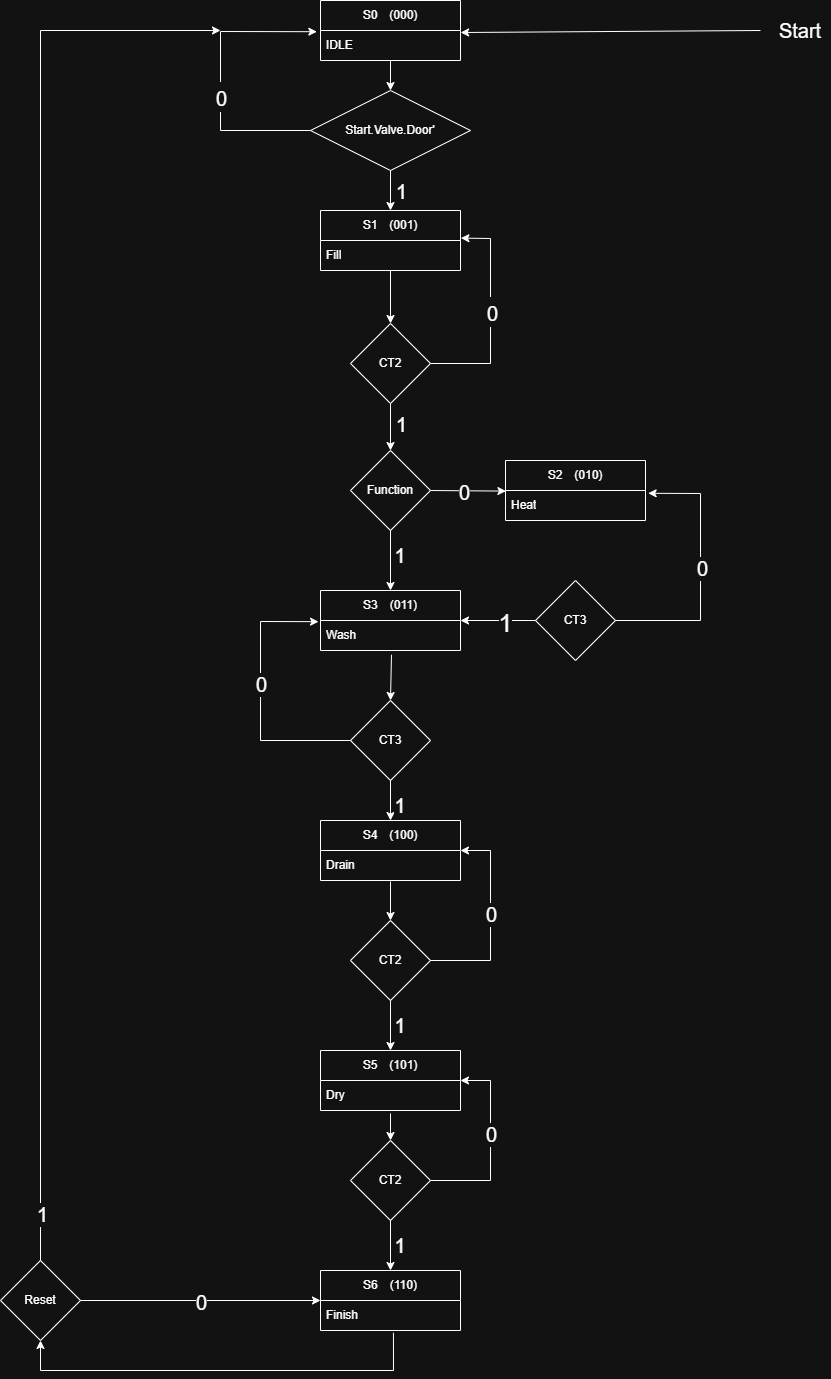
\includegraphics[width=1\textwidth , height = 7.5in]{images/1/1.png}
    \captionof{figure}{َ\lr{ASM Chart} تایمر ماشین لباسشویی}
    \label{fig:1}
\end{center}


\newpage

\subsection{روند پیاده‌سازی}
\label{subsec:imp-detail-1}
\leavevmode\par
\vspace{0.2cm}

\begin{spacing}{1.3}
ابتدا حالت ها را مشخص می‌کنیم. برای این مدار شش حالت زیر را در نظر گرفتیم:
\end{spacing}

\begin{itemize}
\item \lr{$S_0$-Idle (000)}: حالت پایه.
\item \lr{$S_1$-Fill (001)}: آب‌گیری.
\item \lr{$S_2$-Heat (010)}: گرم کردن آب.
\item \lr{$S_3$-Wash (011)}: شست‌وشو.
\item \lr{$S_4$-Drain (100)}: تخلیه.
\item \lr{$S_5$-Dry (101)}: خشک کردن.
\item \lr{$S_6$-Finish (110)}: پایان(در انتظار \lr{Reset}).
\end{itemize}

\begin{spacing}{1.3}
از تراشه 74175 استفاده می‌کنیم که شامل چهار \lr{D-FlipFlop} است، البته ما به فلیپ‌فلاپ چهارم احتیاج نداریم. برای مشخص کردن حالت فعلی مدار، برای هر حالت از یک گیت \lr{AND} استفاده می‌کنیم که ورودی‌های آن \lr{$Q_i$} یا \lr{$\overline{Q_i}$} های متناظر با شماره آن حالت است. برای مثال، یک بودن مقدار \lr{$Q_2 \cdot \overline{Q_1} \cdot Q_0$} متناظر با قرار داشتن در حالت \lr{$S_5$} یعنی خشک کردن است.

حال با استفاده از گیت‌های \lr{AND} دیگری سیگنال‌هایی را تولید می‌کنیم که نشان می‌دهند آیا مجاز به رفتن به حالت بعدی هستیم یا خیر. برای این منظور، سیگنال‌های نشان‌دهنده حالت فعلی مدار را با شرط گذر از آن حالت، یعنی سیگنال های تایمر (\lr{CT2} و \lr{CT3}) \lr{AND} می‌کنیم. برای مثال اگر در حالت شست‌وشو باشیم و از آخرین تغییر حالت مدار سه پالس ساعت گذشته باشد یا به عبارتی \lr{$\text{Wash} \cdot \text{CT3}$} یک باشد، یعنی پالس ساعت بعدی زمان گذر از این حالت به حالت بعدی است.

برای تولید سیگنال‌های \lr{CT2} و \lr{CT3} از تراشه شمارنده 74163 استفاده می‌کنیم. با استفاده از گیت‌های مورد نیاز، سیگنال‌هایی تولید می‌کنیم که وقتی مقدار شمارنده دو و شه باشند یک شود. همچنین پایه \lr{Reset} شمارنده را به ورودی ریست و همچنین گیت‌های \lr{AND} که در بخش قبل ساختیم متصل می‌کنیم. بدین ترتیب، زمانی که کاربر دستوز \lr{Reset} را وارد کند، یا زمان ماندن در یک حالت به اتمام برسد، شمارنده ریست می‌شود.
\end{spacing}

\newpage

\subsection{شماتیک نهایی مدار}
\label{subsec:imp-detail-1}
\leavevmode\par
\vspace{0.2cm}

\begin{center}
    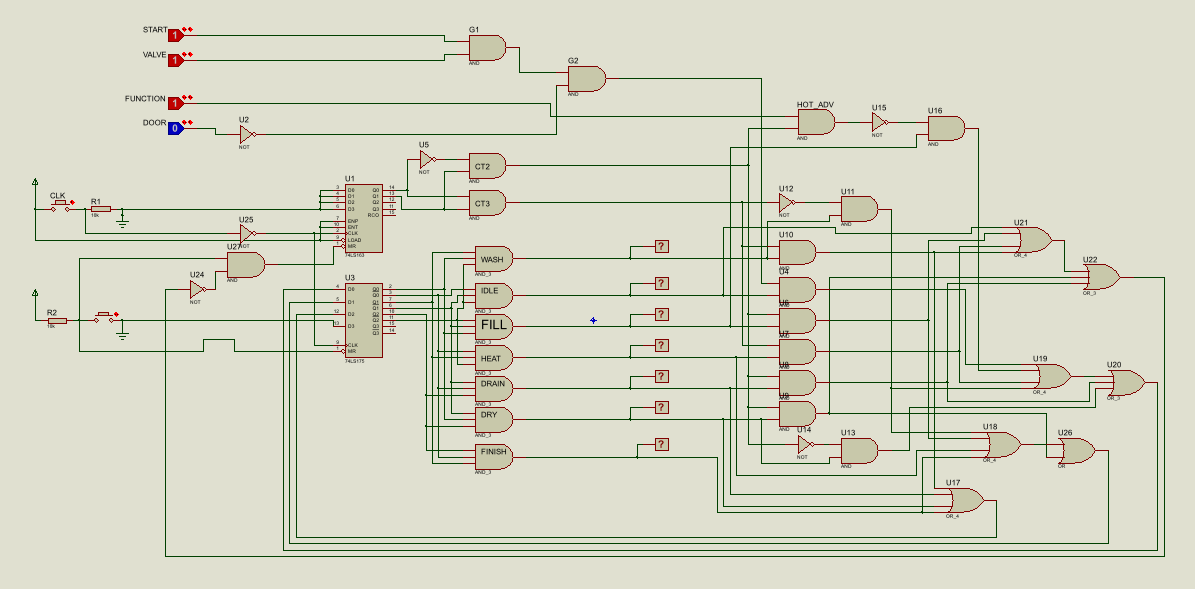
\includegraphics[width=1\textwidth]{images/1/circ.png}
    \captionof{figure}{مدار تایمر ماشین لباسشویی}
    \label{fig:2}
\end{center}

\subsection{بررسی \lr{Test Case} ها}
\label{subsec:imp-detail-1}
\leavevmode\par
\vspace{0.2cm}

\begin{center}
    
\includegraphics[width=1\textwidth]{images/1/t1.png}
    \captionof{figure}{قبل از شروع شست‌وشو}
\end{center}

\begin{center}
    
\includegraphics[width=1\textwidth]{images/1/t2.png}
    \captionof{figure}{شروع شست‌وشو با آب گرم}
\end{center}

\begin{center}
    
\includegraphics[width=1\textwidth]{images/1/t3.png}
    \captionof{figure}{بعد از 3 پالس ساعت}
\end{center}

\begin{center}
    
\includegraphics[width=1\textwidth]{images/1/t4.png}
    \captionof{figure}{بعد از 4 پالس ساعت}
\end{center}

\begin{center}
    
\includegraphics[width=1\textwidth]{images/1/t5.png}
    \captionof{figure}{بعد از فشردن دکمه \lr{Reset}}
\end{center}

\begin{center}
    
\includegraphics[width=1\textwidth]{images/1/t6.png}
    \captionof{figure}{شروع شست‌وشو با آب سرد}
\end{center}

\begin{center}
    
\includegraphics[width=1\textwidth]{images/1/t7.png}
    \captionof{figure}{پس از 3 پالس ساعت}
\end{center}

\begin{center}
    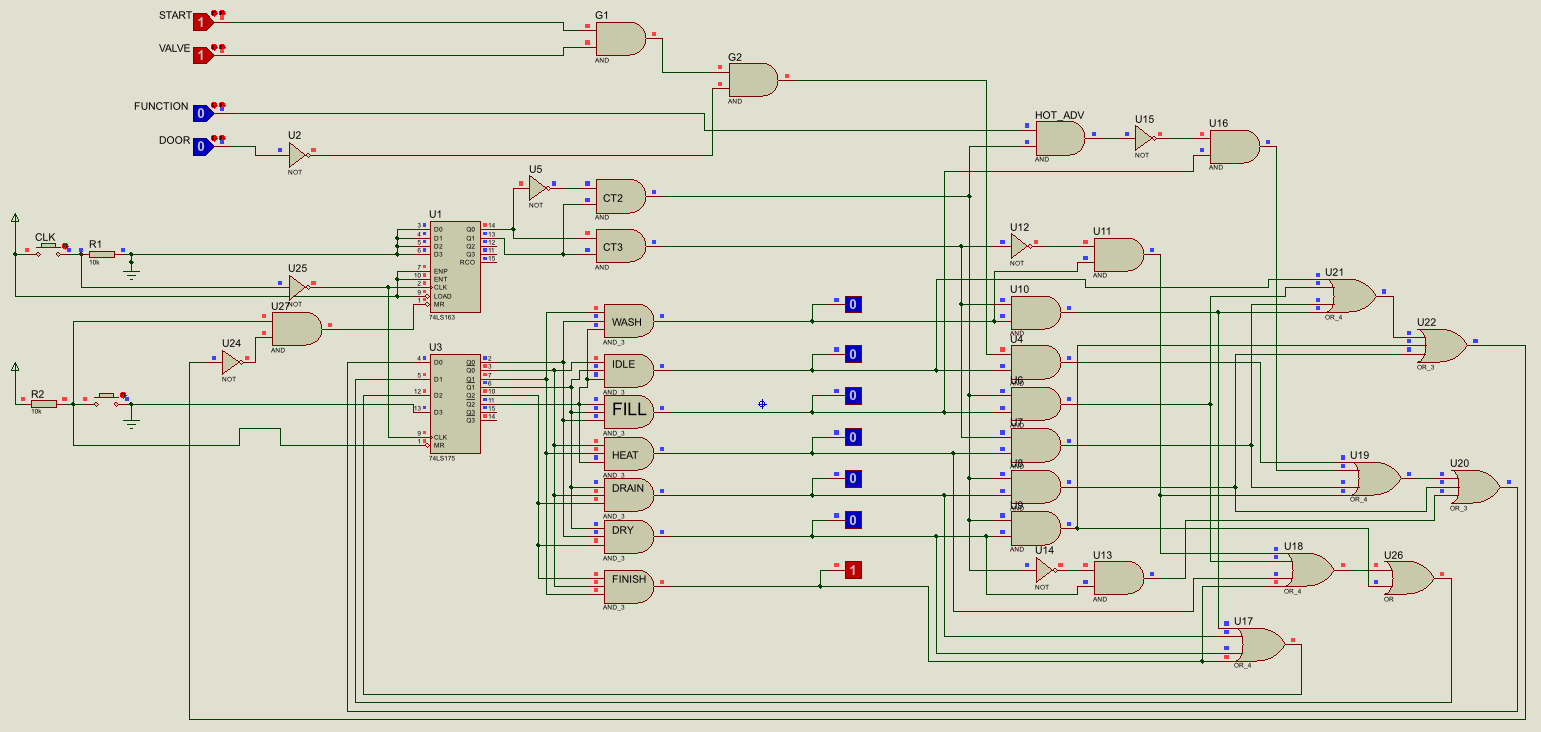
\includegraphics[width=1\textwidth]{images/1/t8.png}
    \captionof{figure}{رسیدن به حالت پایان شست‌وشو}
\end{center}

\newpage

\section{تلفن راه دور}
\leavevmode\par
\vspace{0.3cm}

\subsection{بررسی و انتخاب روش طراحی}
\leavevmode\par
\vspace{0.2cm}

\begin{spacing}{1.3}
برای این مدار نیز مانند مدار قبلی از \lr{ASM Chart} استفاده خواهیم کرد. اما در بخش پیاده‌سازی مدار، به جای طراحی عادی با فلیپ‌فلاپ، از روش \lr{One-Hot} استفاده می‌کنیم.

در این روش، به هر حالت یک فلیپ‌فلاپ اختصاص داده می‌شود و در هر زمان تنها یکی از فلیپ‌فلاپ‌ها مقدار یک دارد که نشان‌دهنده حالت مدار در آن زمان است. اگرچه استفاده از این روش به فلیپ‌فلاپ‌های بیشتری نیاز دارد اما به این دلیل که پیچیدگی طراحی را بسیار کمتر می‌کند و معادلات ورودی فلیپ‌فلاپ‌ها خیلی ساده‌تر می‌شوند، در بسیاری مواقع به‌صرفه است. مخصوصا در مدارهایی که تعداد حالات آنها زیاد نیست اما انتقالات بین حالات پیچیده و تعداد ورودی‌ها زیاد است.
\end{spacing}


\subsection{بلوک‌دیاگرام اولیه}
\label{subsec:imp-detail-1}
\leavevmode\par
\vspace{0.2cm}


\begin{spacing}{1.3}
برای ساختن این مدار \lr{ASM Chart} شکل \ref{fig:tel-asm} را طراحی کردیم. دقت کنید که سیگنال \lr{A} نشان‌دهنده موجودی بزرگتر از صفر است. برای ساخت آن کافی است تمام بیت‌های شمارنده‌ها را با هم \lr{OR} کنیم.
\end{spacing}


\begin{center}
    
\includegraphics[width=1\textwidth]{images/2/1.png}
    \captionof{figure}{\lr{ASM Chart} مدار تلفن}
   	\label{fig:tel-asm}
\end{center}


\subsection{روند پیاده‌سازی}
\label{subsec:imp-detail-1}
\leavevmode\par
\vspace{0.2cm}

\begin{spacing}{1.3}
ابتدا حالت ها را مشخص می‌کنیم. برای این مدار چهار حالت زیر را در نظر گرفتیم:
\end{spacing}

\begin{itemize}
\item \lr{$S_0$-Idle (0001)}: حالت پایه.
\item \lr{$S_1$-Call (0010)}: حالت تماس. چراغ تماس روشن و چراغ هشدار خاموش است.
\item \lr{$S_2$-Alarm (0100)}: حالت هشدار. علاوه بر چراغ تماس، چراغ هشدار نیز روشن می‌شود.
\item \lr{$S_3$-Diconnect (1000)}: قطع‌شدن تماس. به دلیل عدم افزایش موجودی، چراغ تماس خاموش شده و چراغ هشدار روشن می‌ماند و تا زمانی که دکمه \lr{Reset} فشار داده نشود، مدار در همین وضعیت باقی خواهد ماند.
\end{itemize}

\begin{spacing}{1.3}
برای ساختن سیگنال‌های تایمر (\lr{$T_1$} و \lr{$T_2$})، از یک فلیپ‌فلاپ و یک شمارنده دودویی استفاده می‌کنیم. با وصل کردن معکوس خروجی(\lr{$\overline{Q}$}) یک \lr{D-FlipFlop}، خروچی(\lr{$Q$}) آن یک پالس ساعت در میان تغییر می‌کند. از این ویزگی می‌توان برای ساخت سیگنال \lr{$T_1$} استفاده کرد. برای تولید \lr{$T_2$} نیز از تراشه شمارنده 74193 استفاده میکنیم. هرگاه خروجی پایه \lr{$Q_1$} آن از صفر به یک برسد، با در نظر گرفتن یک پالس تاخیر فلیپ‌فلاپ، نشان‌دهنده گذشتن سه پالس ساعت است.

همان‌طور که اشاره شد، در روش \lr{One-Hot} بدست آوردن معادلات ورودی فلیپ‌فلاپ‌ها کار راحتی است. کافی است به فلش‌هایی که به هر حالت وارد می‌شوند دقت کنیم و از آن‌ها اجتماع بگیریم. برای مثال برای فلیپ‌فلاپ نماینده حالت \lr{$S_2$} داریم:
\end{spacing}

$$D_2 = Q_1 \cdot T_1 \cdot \overline{A} + Q_2 \cdot \overline{T_2} \cdot \overline{A}$$


\begin{spacing}{1.3}
و به طریق مشابه معادلات ورودی هر چهار فلیپ‌فلاپ را بدست می‌آوریم.

در نهایت شمارنده‌های 74192 را به \lr{7-Segment} ها و به یکدیگر متصل می‌کنیم. دکمه افزودن سکه را قرار داده و به کلاک \lr{Up} شمارنده رقم یکان متصل می‌نماییم.
\end{spacing}

\newpage

\subsection{شماتیک نهایی مدار}
\label{subsec:imp-detail-1}
\leavevmode\par
\vspace{0.2cm}


\begin{center}
    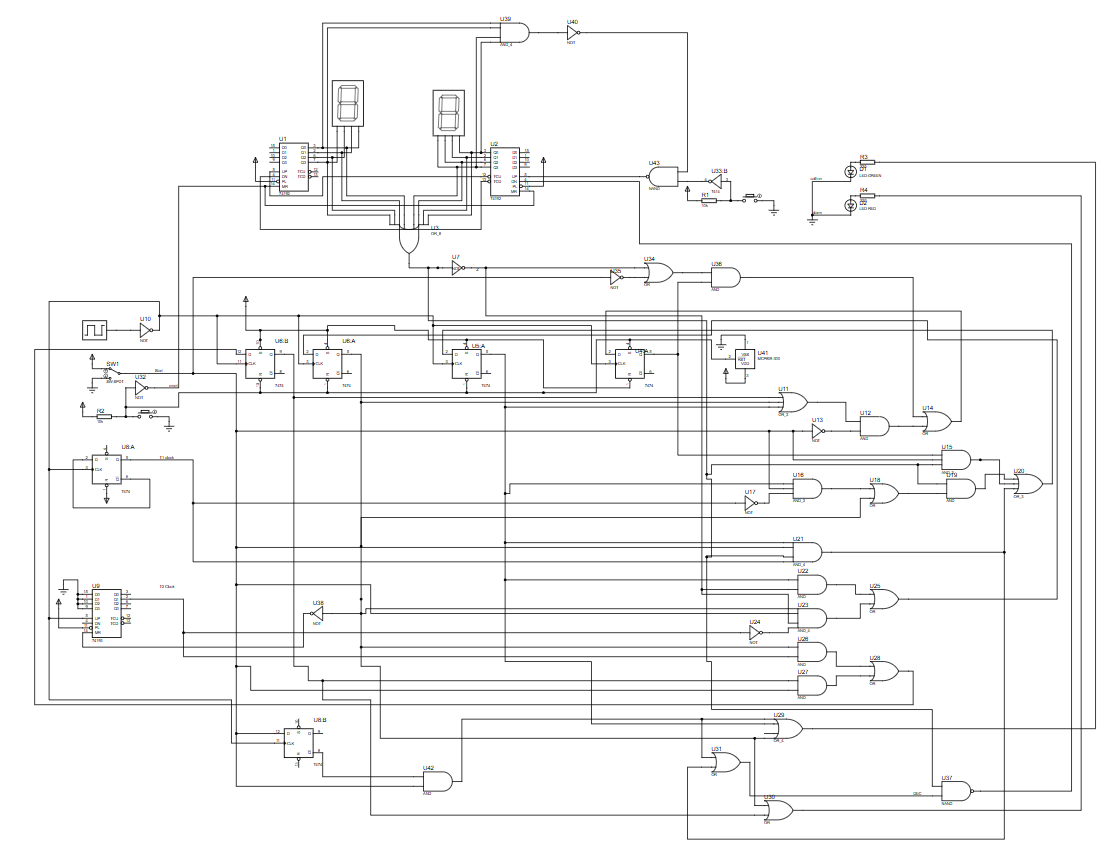
\includegraphics[width=1\textwidth]{images/2/2.png}
    \captionof{figure}{مدار تایمر تلفن}
    \label{fig:2}
\end{center}

\newpage

\subsection{بررسی \lr{Test Case} ها}
\label{subsec:imp-detail-1}
\leavevmode\par
\vspace{0.2cm}

\begin{center}
    
\includegraphics[width=1\textwidth]{images/2/t1.png}
    \captionof{figure}{حالت پایه}
\end{center}

\begin{center}
    
\includegraphics[width=1\textwidth]{images/2/t2.png}
    \captionof{figure}{افرایش سکه}
\end{center}

\begin{center}
    
\includegraphics[width=1\textwidth]{images/2/t3.png}
    \captionof{figure}{شروع تماس}
\end{center}

\begin{center}
    
\includegraphics[width=1\textwidth]{images/2/t4.png}
    \captionof{figure}{کم شدن موجودی با گذر زمان (طی شدن پالس‌های ساعت)}
\end{center}

\begin{center}
    
\includegraphics[width=1\textwidth]{images/2/t5.png}
    \captionof{figure}{ورود به حالت هشدار}
\end{center}

\begin{center}
    
\includegraphics[width=1\textwidth]{images/2/t6.png}
    \captionof{figure}{قطع‌شدن تماس بعد از عدم افرزایش موجودی}
\end{center}

\begin{center}
    
\includegraphics[width=1\textwidth]{images/2/t7.png}
    \captionof{figure}{پس از \lr{Reset}}
\end{center}


\section{نتیجه‌گیری}
\leavevmode\par
\vspace{0.3cm}


\begin{spacing}{1.3}
در این آزمایش، طراحی و پیاده‌سازی مدارهای کنترل‌کننده دیجیتال با استفاده از \lr{ASM Chart} و شبیه‌سازی آن‌ها در نرم‌افزار \lr{Proteus} با موفقیت مورد ارزیابی قرار گرفت. انجام همزمان هر دو پروژه نشان داد که نمودارهای \lr{ASM} ابزاری بسیار کارآمد برای مدل‌سازی ماشین‌های حالت و کنترل سیستم‌های دارای زمان‌بندی و شروط مختلف هستند.

در پروژه اول (تایمر ماشین لباس‌شویی)، مشاهده کردیم که کنترل‌کننده توانست با بررسی دقیق ورودی‌های ایمنی (مانند وضعیت شیر آب و بسته بودن در) و بر اساس برنامه انتخابی (آب گرم یا سرد)، توالی زمانی دقیق عملیات شامل آب‌گیری، گرم کردن، شست‌وشو، تخلیه و خشک کردن را به درستی و بر اساس پالس‌های ساعت مدیریت کند. 

در پروژه دوم (تلفن راه‌دور)، عملکرد مدار در زمینه دریافت، شمارش و نمایش سکه‌های ده ریالی بر روی نمایشگرهای ۷ قطعه‌ای با موفقیت آزمایش شد. نتایج شبیه‌سازی نشان داد که کنترل‌کننده به خوبی قادر است کسر موجودی در طول زمان برقراری تماس (\lr{Call})، فعال‌سازی به‌موقع چراغ هشدار (\lr{Alarm}) در هنگام صفر شدن موجودی و در نهایت قطع مکالمه در صورت عدم ورود سکه جدید را پیاده‌سازی نماید.

به طور کلی، این آزمایش فرایند گام‌به‌گام تبدیل یک سناریوی توصیفی پیچیده به یک نمودار الگوریتمی سخت‌افزاری را به خوبی نشان داد و نقش حیاتی مدارهای کنترل‌کننده در هماهنگ‌سازی و اجرای دقیق دستورات در سیستم‌های دیجیتال را به طور عملی اثبات نمود.

\end{spacing}


\end{document}